\begin{figure*}[t]
{
%\vspace{-0.2in}

%\centering
{
%\begin{minipage}[t]{.31\linewidth}
%\centering
%{
%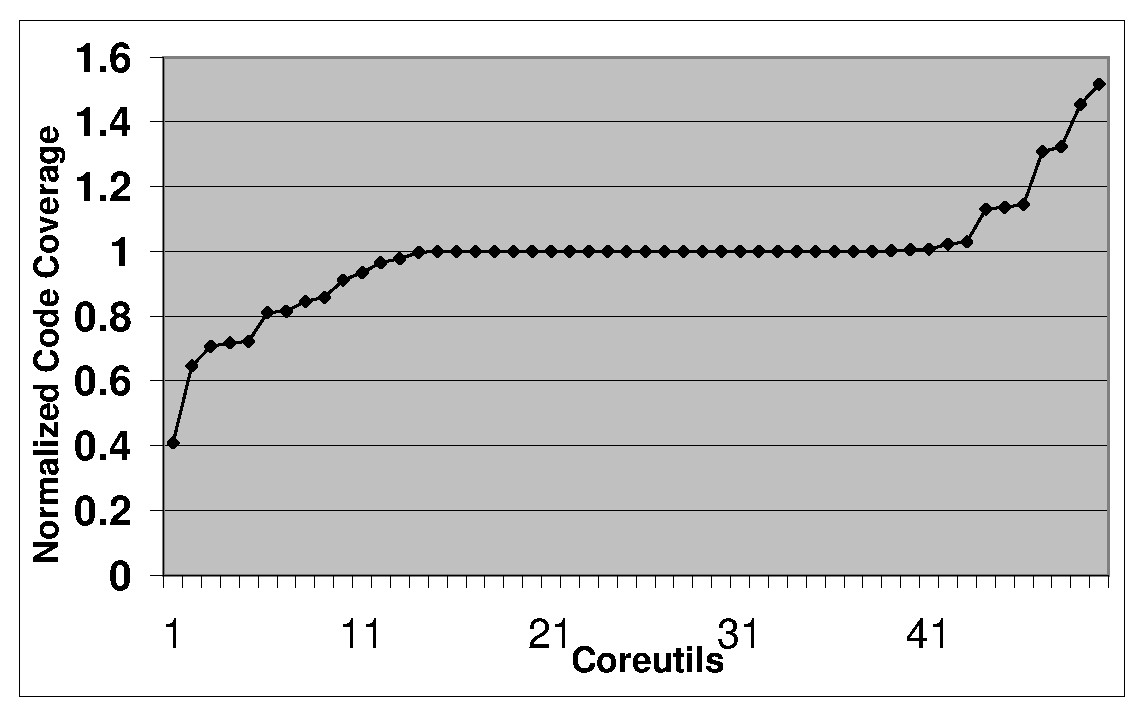
\includegraphics[width=2.1in]{figures/EPS/klee-coverage.eps}
%\caption{\scriptsize{\textit{Normalized code coverage in coreutils binaries as compared to source }}}
%\label{fig:KleeCovRes}
%}
%\end{minipage}

\begin{minipage}{.24\linewidth}
%\centering
{
\begin{scriptsize}
\begin{tabular}{|l|l|} %|r|r|r|}
%xxxxx\=xxxxxxxxxxxxx\=xxxxxx\=xxxxxxxxxxx\=xxxxxx\=  \kill\\
\hline
{mkdir -Z a b}&{mkdir -Z @@ -}\\ 
{mkfifo -Z a b}&{mkfifo -Z @@ -}\\ 
{mknod -Z a b p}&{mkdir -Z @@ - p@}\\ 
{seq -f \%0 1}&{seq -f \%1 1}\\ 
{paste -d\textbackslash \textbackslash   }&{paste -d\textbackslash \textbackslash   }\\ 
{\hspace{1ex}abcdefghijklmn}&{\hspace{1ex}@@@@@@@@ }\\ 
{}&{\hspace{1ex}@@@@@@ }\\  \hline
\end{tabular}
\caption {{\textit{Testcases for crashes (a)Source code~\cite{Cadar-KLEE} (b) Binaries }}}
\label{fig:result-symExec-testCases}
\end{scriptsize}%\vspace{-4ex}
}
\end{minipage}
%\begin{minipage}{.24\linewidth}
%\centering
%{
%\includegraphics[width=\linewidth]{figures/EPS/resultssymExecution-testCase.eps}
%\caption{{\textit{Test cases for crashes (a) Source code (b) Binaries}}}
%\label{fig:result-symExec-testCases}
%}
%\end{minipage}
\hfill
\hspace{1ex}
\begin{minipage}{.21\linewidth}
\centering
{
\begin{scriptsize}
\begin{tabular}{|l|l|l|} %|r|r|r|}
%xxxxx\=xxxxxxxxxxxxx\=xxxxxx\=xxxxxxxxxxx\=xxxxxx\=  \kill\\
\hline
{Binary}&{No}&{With}\\ 
{}&{Promotion}&{Promotion}\\ \hline
htget&980&4671\\ \hline
cut&1301&5103\\ \hline
split&1623&4104\\ \hline
\end{tabular}
\caption {{\textit{Improvement in constraints processing with symbol promotion }}}
\label{fig:results-symExecSymMem}
\end{scriptsize}%\vspace{-4ex}
}
\end{minipage}
\hfill
\hspace{1ex}
\begin{minipage}{.24\linewidth}
\centering
{
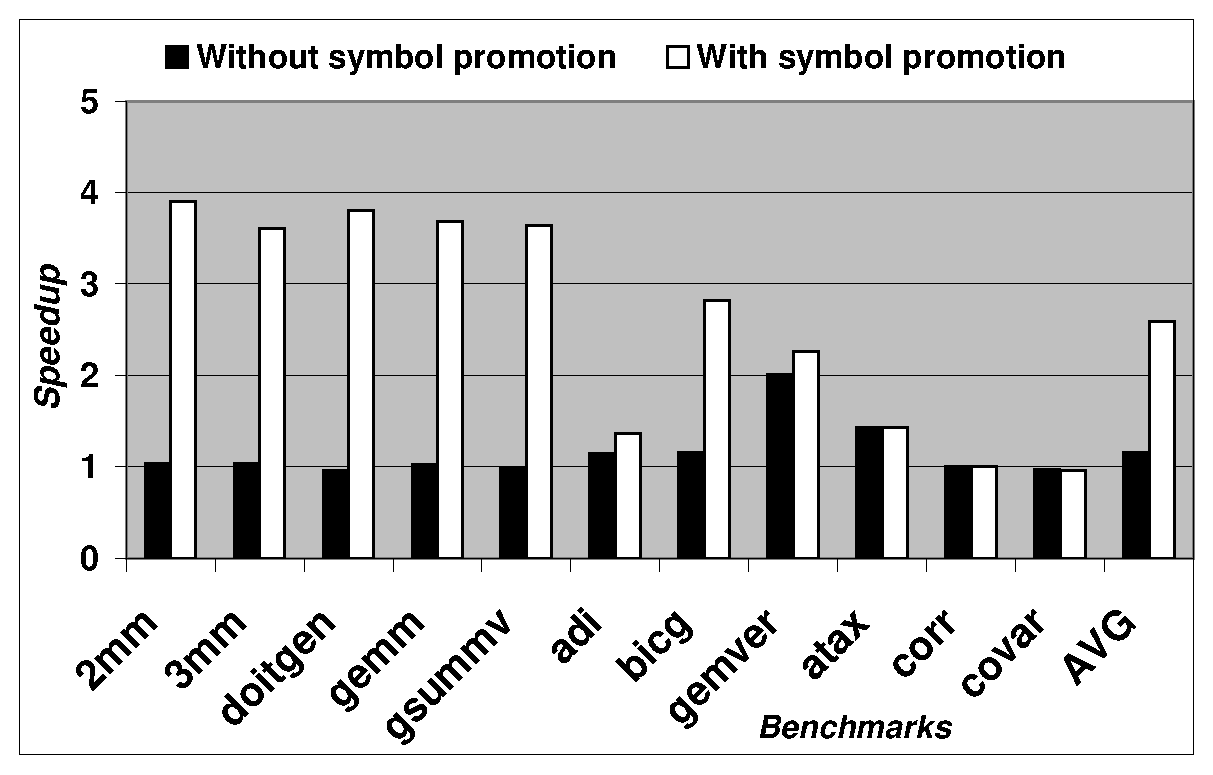
\includegraphics[width=\linewidth]{figures/EPS/parallel-runtime.eps}
\caption{{\textit{Automatic parallelization}}}
\label{fig:parallel-runtime}
}
\end{minipage} 
\hfill
%\hspace{-2ex}
\begin{minipage}{.24\linewidth}
\centering
{
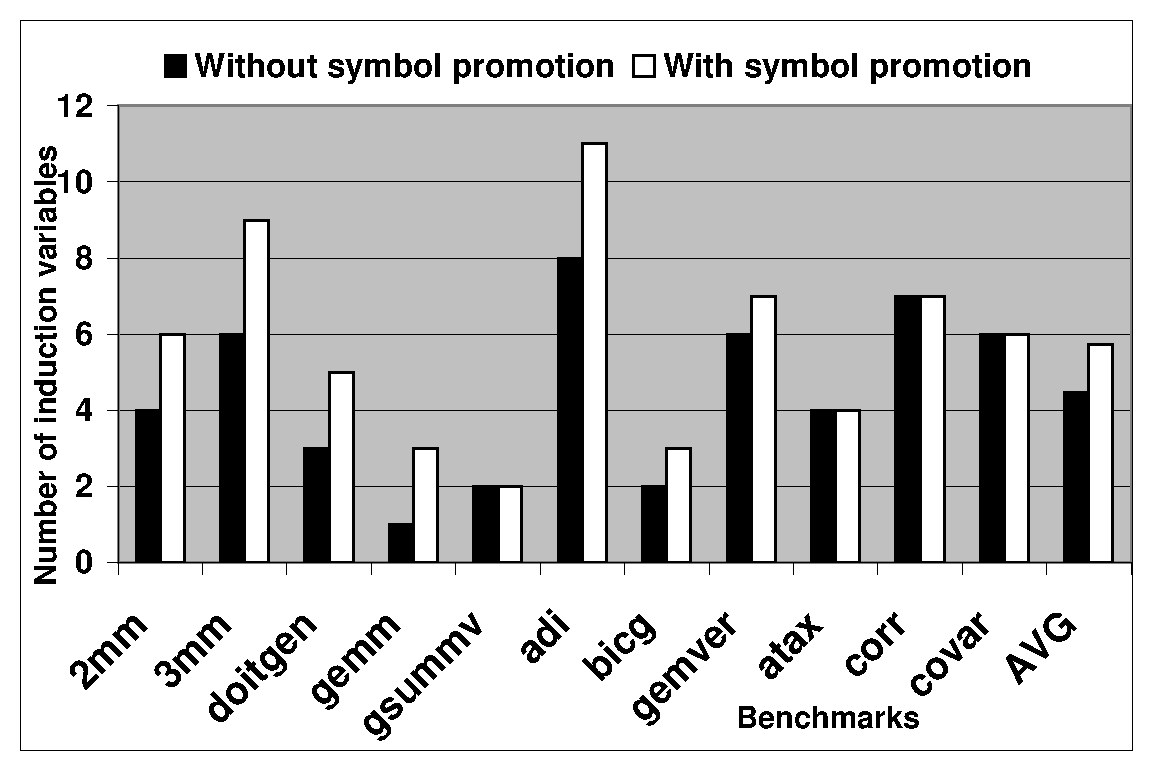
\includegraphics[width=\linewidth]{figures/EPS/induction-var.eps}
\caption{{\textit{Number of induction variables recognized}}}
\label{fig:parallel-indvar}
}
\end{minipage}
}
\vspace{-3ex}
}
\end{figure*}
